%%%%%%%%%%%%%%%%%%%%%%%%%%%%%%%%%%%%%%%%%
% Short Sectioned Assignment
% LaTeX Template
% Version 1.0 (5/5/12)
%
% This template has been downloaded from:
% http://www.LaTeXTemplates.com
%
% Original author:
% Frits Wenneker (http://www.howtotex.com)
%
% License:
% CC BY-NC-SA 3.0 (http://creativecommons.org/licenses/by-nc-sa/3.0/)
%
%%%%%%%%%%%%%%%%%%%%%%%%%%%%%%%%%%%%%%%%%

%----------------------------------------------------------------------------------------
%	PACKAGES AND OTHER DOCUMENT CONFIGURATIONS
%----------------------------------------------------------------------------------------

\documentclass[paper=a4, fontsize=11pt]{scrartcl} % A4 paper and 11pt font size

\usepackage[T1]{fontenc} % Use 8-bit encoding that has 256 glyphs
\usepackage{fourier} % Use the Adobe Utopia font for the document - comment this line to return to the LaTeX default
\usepackage[english]{babel} % English language/hyphenation
\usepackage{amsmath,amsfonts,amsthm} % Math packages
\usepackage{graphicx}
\usepackage{lipsum} % Used for inserting dummy 'Lorem ipsum' text into the template
\usepackage{subfigure}
\usepackage{sectsty} % Allows customizing section commands
\allsectionsfont{\centering \normalfont\scshape} % Make all sections centered, the default font and small caps
\usepackage{setspace}
\usepackage{indentfirst}
\usepackage{fancyhdr} % Custom headers and footers
\pagestyle{fancyplain} % Makes all pages in the document conform to the custom headers and footers
\fancyhead{} % No page header - if you want one, create it in the same way as the footers below
\fancyfoot[L]{} % Empty left footer
\fancyfoot[C]{} % Empty center footer
\fancyfoot[R]{\thepage} % Page numbering for right footer
\renewcommand{\headrulewidth}{0pt} % Remove header underlines
\renewcommand{\footrulewidth}{0pt} % Remove footer underlines
\setlength{\headheight}{13.6pt} % Customize the height of the header

\numberwithin{equation}{section} % Number equations within sections (i.e. 1.1, 1.2, 2.1, 2.2 instead of 1, 2, 3, 4)
\numberwithin{figure}{section} % Number figures within sections (i.e. 1.1, 1.2, 2.1, 2.2 instead of 1, 2, 3, 4)
\numberwithin{table}{section} % Number tables within sections (i.e. 1.1, 1.2, 2.1, 2.2 instead of 1, 2, 3, 4)

\setlength\parindent{0pt} % Removes all indentation FROM paragraphs - comment this line for an assignment with lots of text
% \doublespacing
\linespread{1.6}

\setlength{\parskip}{8pt}

%----------------------------------------------------------------------------------------
%	TITLE SECTION
%----------------------------------------------------------------------------------------

\newcommand{\horrule}[1]{\rule{\linewidth}{#1}} % Create horizontal rule command with 1 argument of height

\title{	
\normalfont \normalsize 
\textsc{EECS332 Project Report} \\ [25pt] % Your university, school and/or department name(s)
\horrule{0.5pt} \\[0.4cm] % Thin top horizontal rule
\huge Who's in My Photo? \\ % The assignment title
\normalsize detect and recognize faces in photos
\horrule{2pt} \\[0.5cm] % Thick bottom horizontal rule
}

\author{Qinglin Li, qlt073} % Your name

\date{\normalsize\today} % Today's date or a custom date

\begin{document}

\maketitle % Print the title

\textit{Course review related information(My views of computer vision, what I learned and feedbacks) can be found behind the reference section}

\section{Introduction}

We all take photos a lot with our friends and our family. It will be very exciting to let the computer automatically recognize the people in a photo. In this project, we want to detect the faces in a given photo and recognize the registered faces whilst labeling the unregistered faces as unknown. For example, Figure \ref{fig:intro_recog} shows a photo of me, my teammate Geng and a friend of us whose face is not registered. The computer correctly detected and recognized the faces of me and Geng as ourselves(in green rectangles with our names) while labeling the face of our unregistered friend as unknown(in red rectangle).
\newpage
\begin{figure}[!htbp]
	\centering
	\subfigure[Original photo]{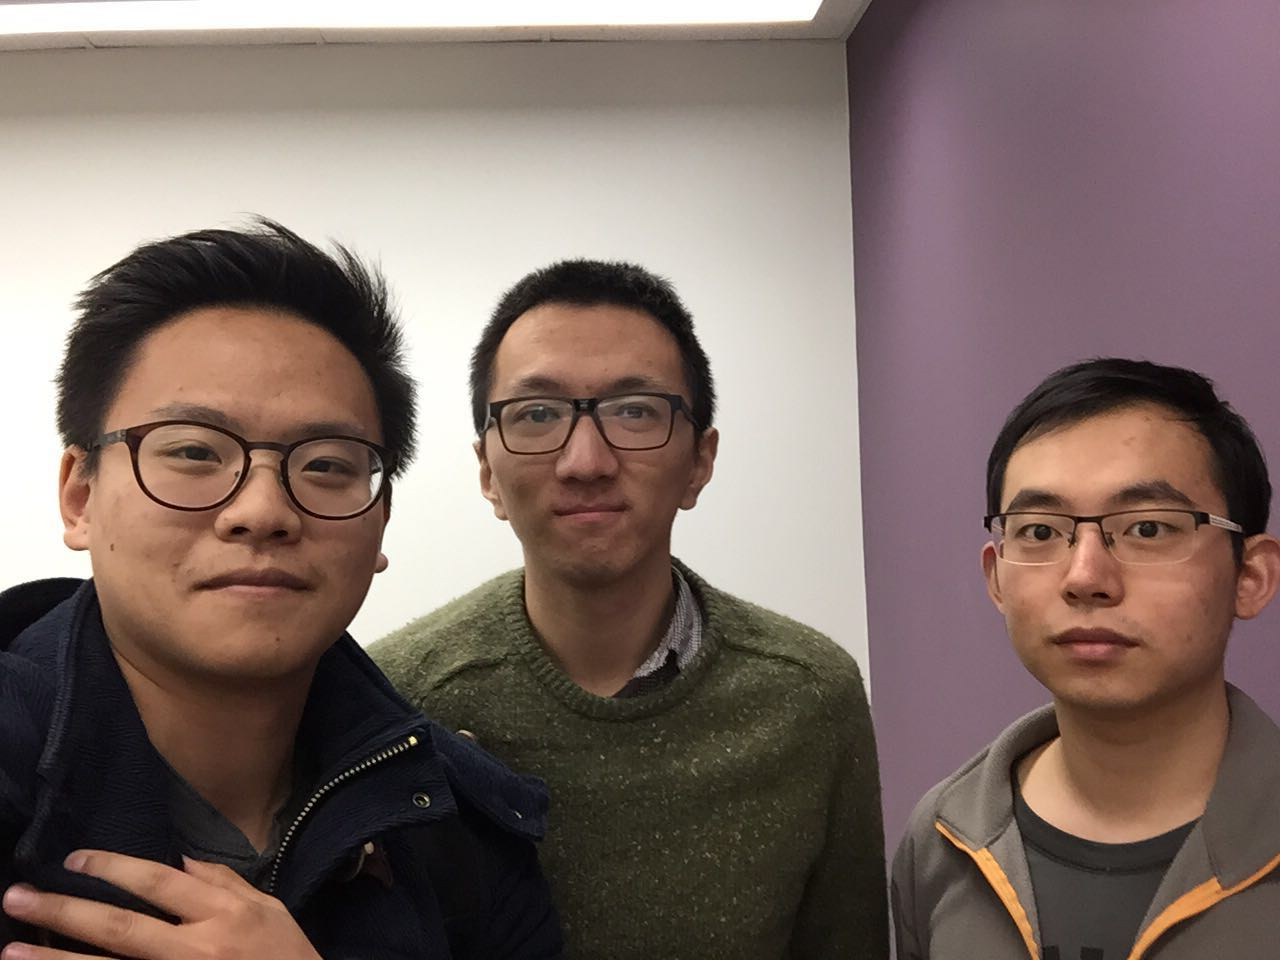
\includegraphics[scale=0.2]{test1.jpg}}
	\subfigure[Photo with faces recognized]{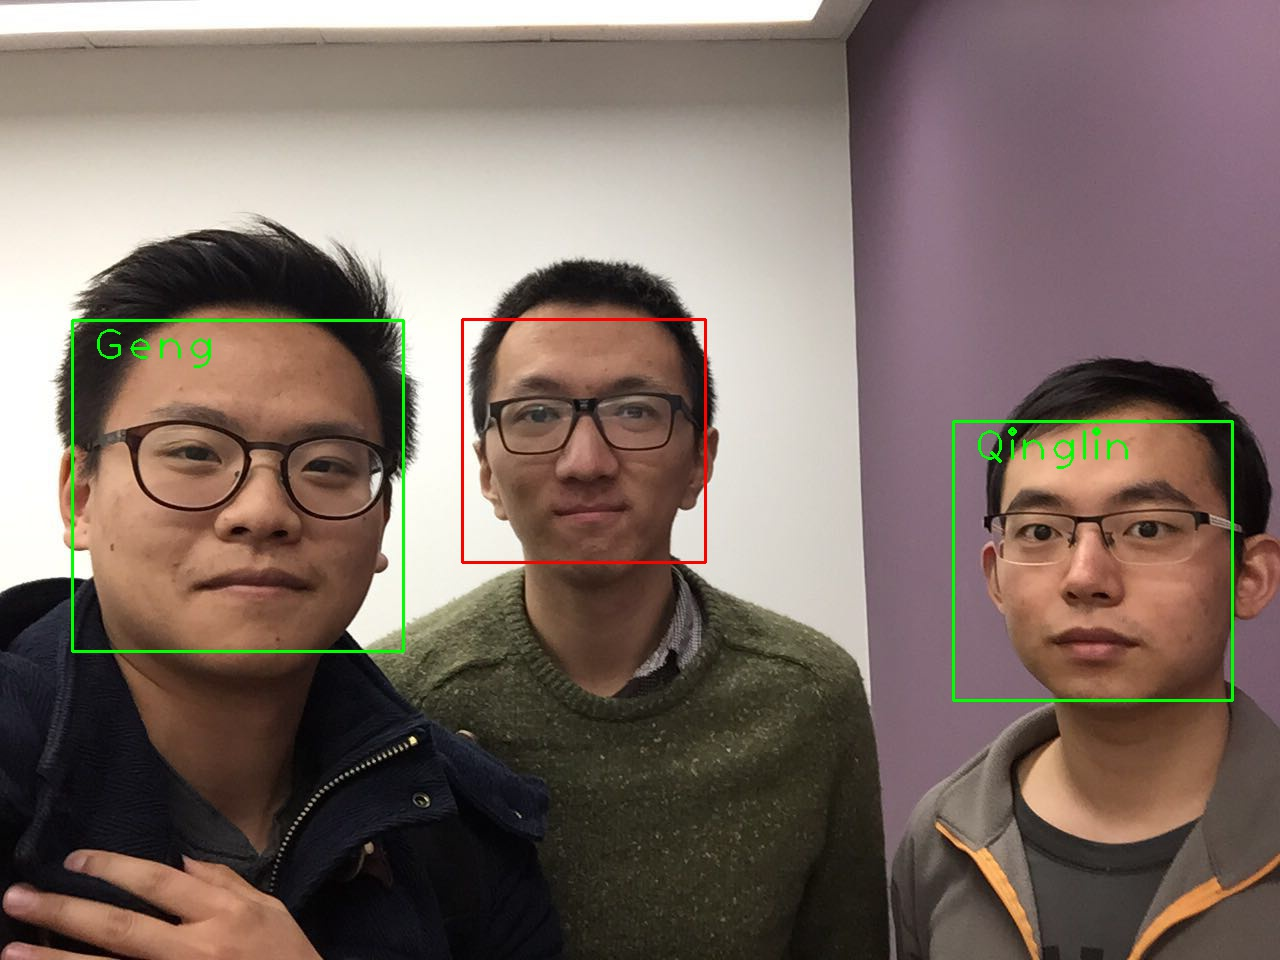
\includegraphics[scale=0.2]{test1_rec.jpg}}
	\caption{A photo of me, Geng and a unregistered friend. (a) shows the original photo and (b) shows the recognition result.}
	\label{fig:intro_recog}
\end{figure}

The whole process of our project could be divided into two stages: registration and matching. In registration stage, we collect photo of our users and crop their faces. After the faces of our users are registered, we can do matching. For a given photo, we first detect the faces in the photo. For each detected face, we then extract features and compare the features with registered faces. Finally, we use a greedy based strategy to match the detected faces to registered persons. We also set a threshold to avoid matching unregistered faces in the photo to registered persons not shown in the photo.

\section{Division of Labor}
The most important part of our project is feature extraction. In our presentation, we mentioned two methods -- Eigenface\cite{turk1991face} and LBP histogram\cite{ahonen2006face} -- for face feature extraction. Since I mainly ran experiments using Local Binary Pattern Histogram(LBPH) and Geng mainly used Eigenface, I'll talk more about LBPH in my report. I also implemented the face cropping for registration and face detection. They are similar and relatively easy since I used OpenCV's\cite{opencv_library} built-in implementation of Viola and Jones' cascade detector\cite{viola2001rapid}.

\section{Registration}
In the registration stage, we crop the faces from each user's registered photos. We assume there is only one face in each registered photo, which is the user's face. But we don't require the photo is a photo of the user's face. So we need to crop the face from the registered photo. Figure \ref{fig:register_photo} shows an example of the registered photo. The photo on the left is a photo of me with only my face in it and image on the right is the cropped face.

\begin{figure}[!htbp]
	\centering
	\subfigure[A photo of me]{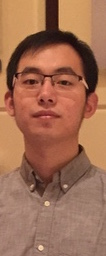
\includegraphics[scale=0.8]{me.jpg}}
	\qquad
	\subfigure[Cropped face]{
\includegraphics[scale=0.8]{myface.jpg}}
	\caption{(a) shows a photo of me as an example and (b) shows the cropped face.}
	\label{fig:register_photo}
\end{figure}

Here, we use OpenCV's CascadeClassifier, which implements Viola and Jones' cascade detector\cite{viola2001rapid}. The training process needs a lot of face and non-face images. It uses Haar like features to train a bunch of weak classifiers and Adaboost is then applied to ensemble the weak classifiers. Its detection process scans sliding windows of different scales and classify if there is a face in the window. The detection process is also accelerated by using the classifiers in a cascade manner. That's why the method is called \textit{Cascade Detector}.

\section{Feature Extraction}
In feature extraction section, we will talk about two classical handcrafted feature for face recognition.
\subsection{Eigenface}
The intuition of Eigenface\cite{turk1991face} is our facial features are always of the similar shapes. So the intensity of the pixels at the corresponding positions should be highly related. So we can use Principle Component Analysis(PCA) to reduce dimension of the data and get the relationships between pixels. Eigenface gives us eigenvectors of the covariance matrix as new basis of the face images under which the distance can reflect the dissimilarity of faces more accurately. The eigenvectors are called Eigenfaces.

Eigenface is a classical yet not bad method for face recognition. It is easy to code and it adequately reduces statistical complexity in face image representation. And once the Eigenfaces are computed, the face recognition could achieve real-time.

However, it also has several critical weakness: It is very sensitive to lighting, scale and translation. It could happen that the most significant Eigenface reflects the lighting changing, which doesn't give us any useful information. So it requires a highly controlled environment.

Eigenface related work in our project is mainly done by my teammate Geng.

\subsection{Local Binary Pattern}

The Local Binary Pattern(LBP) feature is first proposed for texture classification\cite{ojala1996comparative}. And it is then used for face recognition by Ahonen et al\cite{ahonen2006face}. One of the best handcrafted features before deep learning is based on LBP feature\cite{chen2013blessing}.

\begin{figure}[!htbp]
	\centering
	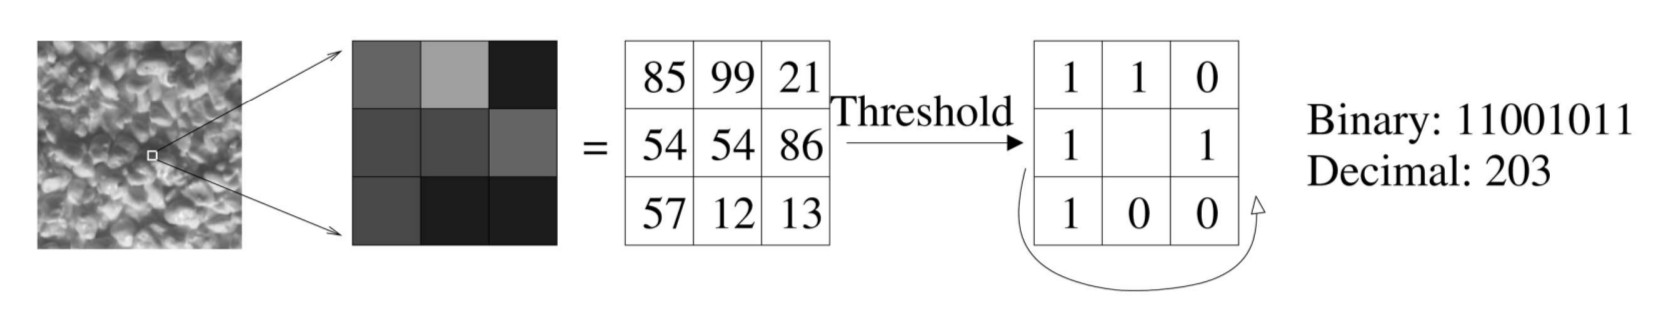
\includegraphics[width=6in]{lbp.png}
	\caption{An example of extracting LBP feature}
	\label{fig:lbp}
\end{figure}

The original LBP operator forms labels for the image pixels comparing each pixel to its 8 neighbors (left-top, left-middle, left-bottom, right-top, etc.)and follow the pixels along a circle, i.e. clockwise or counter-clockwise. If center pixel's value is greater than the neighbor's value, we get a $0$, otherwise, we get a $1$. When comparing each pixel with its 8 neighbors, we can get an 8 bit binary number with $2^8$ possible combinations ranging from $0$ to $255$. An example of LBP is shown in Figure \ref{fig:lbp}. By comparing the center pixel with its neighbors and concatenate all the binary bits, we get a binary code $(11001011)_2$, which is $203$ in decimal number. Actually, we can show the LBP feature as a grayscale image, one example of which is shown in Figure \ref{fig:faces_difflight} and Figure \ref{fig:faces_difflight_lbp}.

\begin{figure}[htbp]
	\centering
	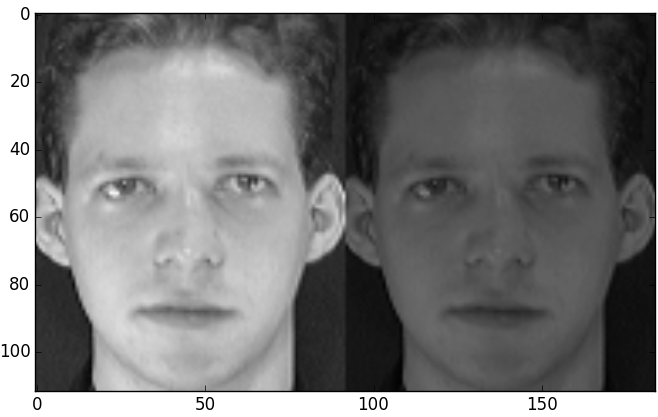
\includegraphics[width=5in]{faces_difflight.png}
	\caption{A face of the same person under different lighting conditions}
	\label{fig:faces_difflight}
\end{figure}

The LPB feature is formally defined as 
$$LBP(x_c, y_c) = \sum_{p = 1}^{P}2^{p-1}\text{sign}\left(I(x_p, y_p) - I(x_c, y_c)\right)$$
Where $x_c, y_c$ indicates the coordinates of the center pixel and $x_p, y_p$ indicates the coordinates of its p-th neighbor, $I(x, y)$ is the intensity of the pixel located at $(x, y)$. $\text{sign}(x)$ is the sign function defined as
$$
\text{sign}(x)=\left\{
	\begin{aligned}
	&1 \quad x\geq 0\\
	&0 \quad \text{otherwise}
	\end{aligned}
	\right.
$$
Since LBP feature reflects the relationship between each pixel and its neighbors, it should be invariant under different lighting conditions.  Figure \ref{fig:faces_difflight} shows images of the same face under different lighting conditions. The darker one is simulated by the original image multiplied by $0.5$.  The LBP feature extracted from the two images in shown in Figure \ref{fig:faces_difflight_lbp}. As we could see, even though the lighting condition is different, the LBP feature extracted is still similar.

\begin{figure}[htbp]
	\centering
	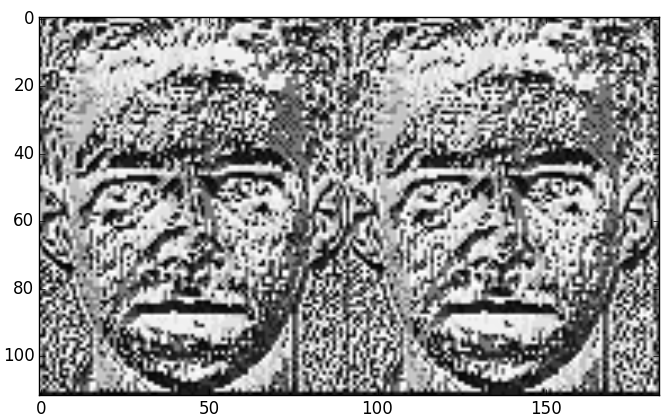
\includegraphics[width=5in]{faces_difflight_lbp.png}
	\caption{Faces in Figure \ref{fig:faces_difflight} after extracting LBP feature(original definition)}
	\label{fig:faces_difflight_lbp}
\end{figure}

To capture the details differs in sizes, the LBP descriptor is then extended to arbitrary size with circular neighborhoods and bilinearly interpolating the pixel values. The extended LBP descriptor has two parameters $P$ and $R$ . $P$ stands for the number of sample points and $R$ is the radius of the circle. This extended LBP descriptor is also called Circular LBP. Here the coordinates of the neighbors is given by
$$
\begin{aligned}
x_p &= x_c + R\cos\left(\frac{2\pi p}{P}\right)\\
y_p &= y_c - R\sin\left(\frac{2\pi p}{P}\right)
\end{aligned}
$$
The intensity of pixel at $(x_p, y_p)$ is computed via bilinear interpolation. Suppose $x_0=floor(x_p), y_0=floor(y_p)$ and $x_1=ceil(x_p), y_1=ceil(y_p)$, $I(x_p, y_p)$  is given by
$$
I(x_p, y_p)=\begin{bmatrix}
x_1 - x_p & x_p - x_0
\end{bmatrix}
\begin{bmatrix}
I(x_0, y_0) & I(x_0, y_1) \\
I(x_1, y_0) & I(x_1, y_1)
\end{bmatrix}
\begin{bmatrix}
y_1 - y_p \\
y_p - y_0
\end{bmatrix}
$$
LBP descriptor itself is still a local description of the image. Using the extracted LBP feature for face recognition is not much different from using raw pixel. To form a global description of the image based on LBP descriptor, we build a histogram. Suppose we've already extracted the LBP feature with parameter $(P, R)$, then the histogram $H$ is given by
$$H_i=\left|\{(x, y)|LBP_{P,R}(x, y)=i\}\right|$$
$|\cdot|$ here stands for set cardinality.

Suggested by the original paper, it's better to split the images into cells, compute the sub-histogram for each cell and then concatenate the sub-histograms into a global histogram. This process is quite like HOG feature\cite{dalal2005histograms}. However, since the detected faces in our project are of different sizes, we only build a normalized global histogram. The LBP histogram of \ref{fig:faces_difflight} is shown in Figure \ref{fig:lbp_hist}. As we could see, the two histograms look similar.

\begin{figure}[htbp]
	\centering
	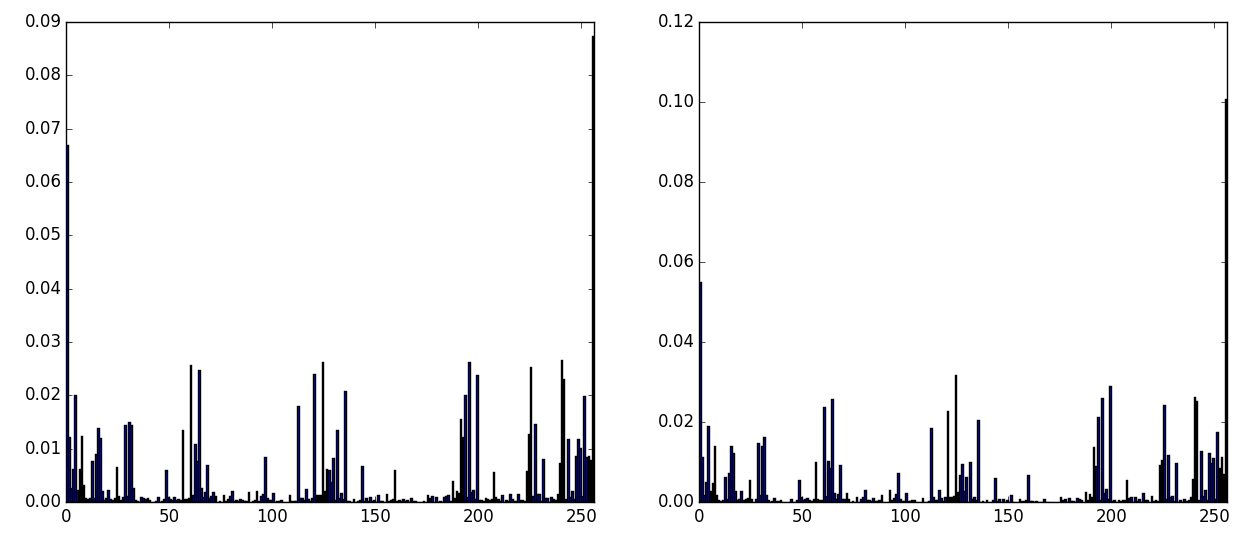
\includegraphics[width=6in]{lbp_hist.png}
	\caption{LBP histograms of Figure \ref{fig:faces_difflight}}
	\label{fig:lbp_hist}
\end{figure}

After the histogram is built, we can then compare two images by compute the dissimilarity between the two corresponding histograms. Comparing two histograms is actually same as comparing distributions. Kullback--Leibler divergence(KL divergence for short, also called relative entropy) and $\chi^2$ statistic are both commonly used metrics. For two distributions/histograms $P$ and $Q$, the KL divergence is defined as
$$KL(P\|Q)=\sum_{i}P_i\log\frac{P_i}{Q_i}$$
And the $\chi^2$ statistic is defined as
$$\chi^2(P\|Q)=\sum_{i}\frac{(P_i - Q_i)^2}{P_i + Q_i}$$
Note that KL divergence is not a symmetric metric, that is $KL(P\|Q)$ not necessarily equals $KL(Q\|P)$. So in order to reduce potential bugs cause by parameter orders, we use $\chi^2$ statistic in practice. 

The $\chi^2$ statistic between the two histogram in Figure \ref{fig:lbp_hist} is $0.021$, which means the dissimilarity is pretty small.

\section{Matching}

For a given photo, suppose all faces in the photo is detected by the cascade detector of OpenCV. For each detected face, we compare it with all registered face of every person, and we only keep the smallest dissimilarity between each detected face and each person. This gives us a dissimilarity matrix. For the case shown in our introduction, a possible dissimilarity matrix is shown in Figure \ref{fig:disimilarity}. This is actually a made up example showing show corner cases.

We assume all the given photos are real photos, so each person can appear at most once in the photo. We match the registered names with detected faces with a greedy strategy: we first sort the dissimilarities, and match the names with detected faces based on the rank of the dissimilarities. If a name or a detected face is already matched, we won't match it again.

In the example shown in Figure \ref{fig:disimilarity}, we first match the name "Qinglin" with the second face, which is mine. Then, the second smallest dissimilarity is between the name "Qinglin" and Geng's face, which is the third one, but since "Qinglin" is already matched with the second face, we will not match "Qinglin" again with Geng's face. In next step, we will match Geng with his own face. And our unregistered friend's face will be labeled as unknown since it cannot be match to any registered person.

\begin{figure}[!htbp]
	\centering
	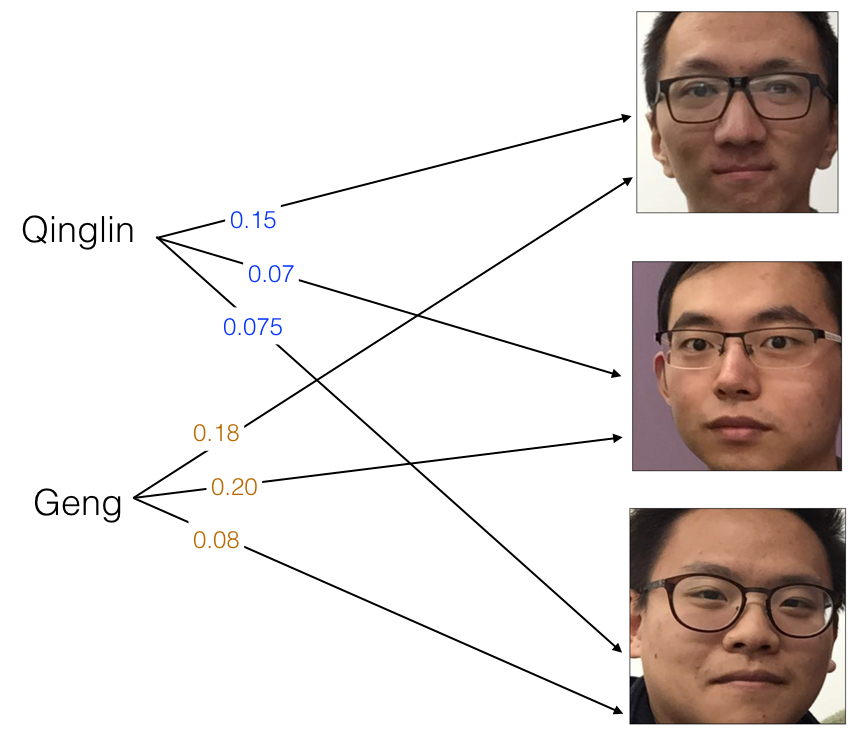
\includegraphics[width=6in]{disimilarity.jpg}
	\caption{An illustration of a dissimilarity matrix}
	\label{fig:disimilarity}
\end{figure}

In practice, if we directly use the method, it would match unregister faces in the photo to registered person not shown in the photo causing a lot of false positives. So we have to set a threshold to reject these cases.

\section{Experiments Settings}
We tested the LBP based recognition method under three cases: recognize single registered person, recognize multiple registered persons in a photo and recognize multiple registered and unregistered persons in a photo. We tested our method on AT\&T face database\cite{Samaria1995Parameterisation}. Some face images could be found in Figure \ref{fig:att_faces}. The database contains $40$ persons and each person has $10$ face images. We made up our own dataset from the AT\&T database to test the last two cases by concatenate the images of single persons together.

\begin{figure}[!htbp]
	\centering
	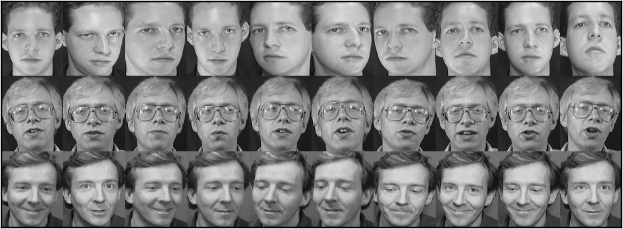
\includegraphics[width=6in]{att_faces.png}
	\caption{Some images from the AT\&T database}
	\label{fig:att_faces}
\end{figure}

We implemented the method with Python2 and the Python interface of OpenCV.

\section{Experiments Results}
\subsection{Experiment 1: Single person recongition}
In this experiment, we split the images of each person as register images and test images. And we simply match each test image to the person with the smallest dissimilarity. This is like a k nearest neighbor classifier with $k=1$. The accuracy curve between different register images number for each person and the accuracy is shown in Figure \ref{fig:acc_single}.

%\newpage
\begin{figure}[!htbp]
	\centering
	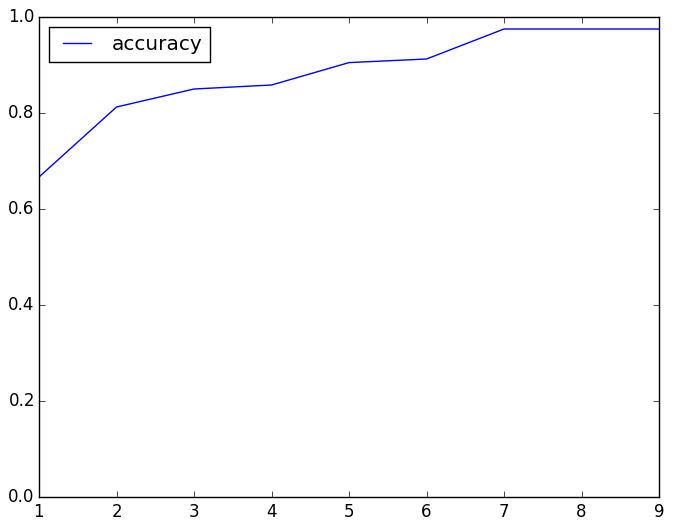
\includegraphics[width=4in]{acc_single.png}
	\caption{Accuracy of different number of register images for each person in experiment 1}
	\label{fig:acc_single}
\end{figure}

We can find that with large number of register images for each person, we are possibly to get a higher accuracy. And with $7$ images registered for each person, we can get a accuracy very close to $100\%$

\subsection{Experiment 2: Detect and recognize multiple registered persons}
This experiment is pretty much similar to the single person recognition experiment. Since everybody in the given photos are registered, we can apply our greedy matching algorithm without using any thresholds. 

A correctly recognized photo of multiple registered persons is shown in Figure \ref{fig:rec_multi_reg}.  Each detected faces in placed in a rectangle box. If a detected face is matched to a registered person, it is labeled by a green box with the person's name in the box. We place a little margin (black region) between each person's images to simulate the distance between persons in real photos.

\begin{figure}[!htbp]
	\centering
	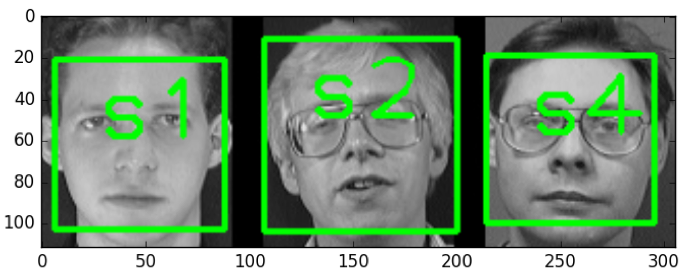
\includegraphics[width=4in]{rec_multi_reg.png}
	\caption{A correctly recognized photo of multiple registered persons}
	\label{fig:rec_multi_reg}
\end{figure}

Since this experiment is almost the same as the last one except for the detection, so the accuracy changes similarly to the last experiment as well. 

\begin{figure}[!htbp]
	\centering
	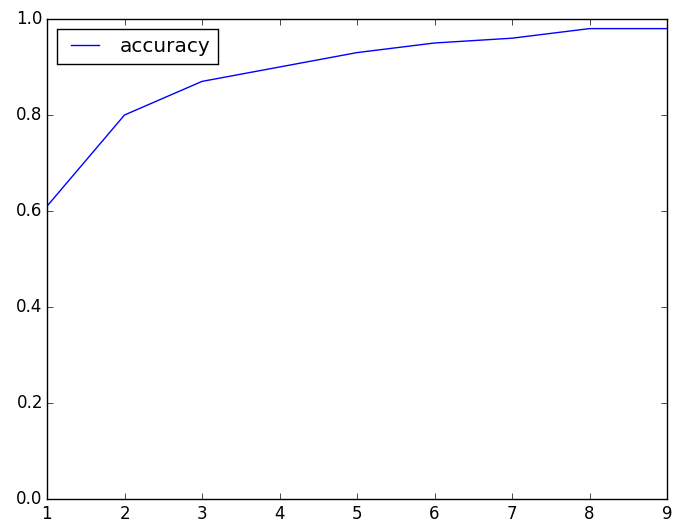
\includegraphics[width=4in]{acc_multi_reg.png}
	\caption{Accuracy of different number of register images for each person in experiment 2}
	\label{fig:acc_multi_reg}
\end{figure}

\subsection{Experiment 3: Detect and recognize multiple registered or unregistered persons}
This experiment is much more challenging. Since somebody in the photo is unregistered, we could easily match these guys to registered but not shown people. So we have to set a threshold to reject these kind of matchings. Currently, we only set a global threshold, any match with a dissimilarity above the threshold will not be considered as a match.

A correctly recognized photo of multiple registered and multiple unregistered persons is shown in Figure \ref{fig:rec_multi_unreg}.  Same as experiment 2, faces in green boxes with names in it is successfully matched faces. And faces in red boxes are faces recognized as unregistered.

\begin{figure}[!htbp]
	\centering
	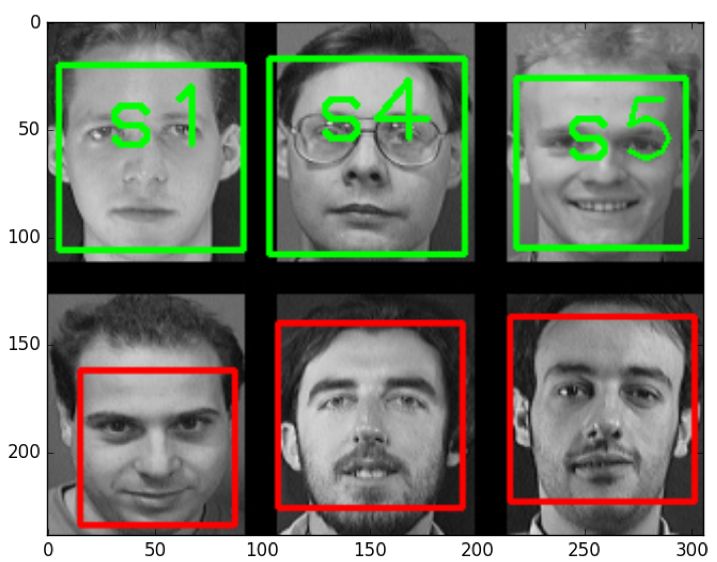
\includegraphics[width=5in]{rec_multi_unreg.png}
	\caption{A correctly recognized photo of multiple registered and multiple unregistered persons}
	\label{fig:rec_multi_unreg}
\end{figure}

We still don't have a good solution to this task. Even if we have $9$ images registered for each person, we can only get a $60\%$--$70\%$ accuracy. Some possible improvements will be discussed in future work section.

\section{Remarks and Future works}
The remarks of our projects are:
\begin{enumerate}
	\item We implemented a system to register the faces of our users and automatically detect and recognize the registered an unregistered faces in given photos
	\item We used the cascade detector for registration and face detection.
	\item We investigated several classical handcrafted features for face recognition.
	\item We tested our method on AT\&T database and we crafted our own dataset from AT\&T dataset.
\end{enumerate}

Nearly every part of our project can be improved:
\begin{enumerate}
	\item For registration, the cascade detection integrated in OpenCV is good enough for front faces. But if the face rotate a little bit, it becomes less accurate. We may use more data to train the detector or use some more state-of-the-art detectors.
	\item For feature extraction, we investigated two kinds of feature. But the experiments are conducted on two features separately. So feature fusion would be a useful future for our project. Besides the classical handcrafted features, it would exciting to explore the deep learning based features like VGG Face\cite{Parkhi15}.
	\item For the matching part, instead of using the greedy matching algorithm, we may use some more well-developed algorithms. Such as Gale-Shapley algorithm for stable matching\cite{gale1962college}.
\end{enumerate}

\section{Conclusion}
In this project, we built a system for automatic face detection and recognition in photos. We used cascade detector for face registration and face detection. And then we applied LBP histograms to extract features of the faces. The detected faces are matched to the registered faces based on a greedy strategy.

Our method have a good performance and single face recognition and recognize multiple registered faces in a photo. However, we still have to improve the accuracy when there are multiple registered faces and multiple unregistered faces in a photo.

\newpage
\bibliographystyle{plain}
\bibliography{references.bib}

\newpage
\section*{Personal views of Computer Vision}
Computer Vision is a field about processing, analyzing and understanding images and videos. It is a very exciting and challenging field. And it is also one of the hottest fields in artificial intelligence.

Computer Vision can be divided into low level vision, middle level vision and high level vision. 

Low level vision mostly focus on image processing and the cameras. It involves understanding the properties and a lot of geometry. For given images, low level vision methods output another image or the properties of the images or corresponding cameras. 

Middle level vision, on the other hand, analyze the geometry of the images or motions. Typical middle level tasks includes region segmentation, stereo and motion analysis. 

Moreover, high level vision understands the images. So it involves a lot of feature extracting and machine learning. Nowadays, with the rising of deep learning, researchers in high level vision tends to use more and more deep (convolutional) neural network models to perform a end-to-end learning and learn feature automatically from massive data.

Computer Vision has many applications. A obvious application of computer vision is on digital cameras. Digital cameras use a lot of computer vision techniques to help users take better photos. Biometrics also uses quite much computer vision for Iris/face/fingerprint recognition or verification. Another main application of computer vision is in robotics and automatic driving. They use computer vision to recognize and understand the environment and make decisions. It is worthy to mention that AlphaGo, Google's go artificial intelligence, which beats the Go world champion, uses deep convolutional neural networks for decision, which is also very often used in computer vision.  Augmented reality and virtual reality can also count as applications of computer vision, since they are actually an intersection of graphics and vision.

\section*{What I learned and what I want to study more}
This course mostly covers low level vision and some middle level vision. It introduce basic concepts such as connected component, histogram equalization, color based segmentation, texture, edge, cameras to some more advanced concepts including face detection, curve fitting, motion estimation, hough transform, image stitching, SIFT and stereo.

This course itself is awesome, but it only covers image processing. However, video processing is also a important topic in low and middle level vision. Basics such as optical flow should also count as low or middle level vision. I also want to learn more about other classical features like HOG, SURF, FAST and Harris corner.

\section*{Feedback and Suggestions}
I quite like this course, but I have the following two suggestions:
\begin{enumerate}
	\item Prof. Wu sometimes spends too much time on some math details. He could just skip them leaving the conclusions and references, so more interesting topics in computer vision could be covered in the course.
	\item Since videos are also important in computer vision, basic video processing technology can also be included in this course.
\end{enumerate}
\end{document}
